\documentclass[conference]{IEEEtran}
\IEEEoverridecommandlockouts
\usepackage{iftex}
\ifXeTeX
  \usepackage{fontspec}
  \setmainfont{texgyretermes}[Extension=.otf,UprightFont=*-regular,BoldFont=*-bold,ItalicFont=*-italic,BoldItalicFont=*-bolditalic,BoldFeatures={Ligatures=NoCommon}]
  \setmonofont{texgyrecursor}[Extension=.otf,UprightFont=*-regular,BoldFont=*-bold,ItalicFont=*-italic,BoldItalicFont=*-bolditalic,BoldFeatures={Ligatures=NoCommon}]
\fi
\usepackage{cite}
\usepackage{amsmath,amssymb}
\usepackage{graphicx}
\usepackage{booktabs}
\usepackage{array}
\usepackage{xcolor}
\usepackage{url}
\usepackage{tikz}
\usetikzlibrary{positioning,arrows.meta}
\usepackage{pgfplots}
\pgfplotsset{compat=1.17}
\usepackage[hidelinks]{hyperref}

\begin{document}
\bstctlcite{IEEEexample:BSTcontrol}

\title{MedGuardian: Deterministic Tools, Pre-Order Verification, and Guideline-Grounded Guardians for Reliable Clinical LLM Agents%
\thanks{Project Code: G3-07, AI4015 Agentic Artificial Intelligence. Supervisor: Naeem Tareen.}}

\author{
\IEEEauthorblockN{Syed Muhammad Mustafa}
\IEEEauthorblockA{Roll No.\ 23i-0661\\
FAST-NUCES, Islamabad, Pakistan\\
i230661@isb.nu.edu.pk}
\and
\IEEEauthorblockN{Muhammad bin Taimur}
\IEEEauthorblockA{Roll No.\ 23i-0810\\
FAST-NUCES, Islamabad, Pakistan\\
i230810@isb.nu.edu.pk}
}

\maketitle

\begin{abstract}
Large language model (LLM) agents that act on electronic health records perform reasonably well on simple lookups but become unreliable once they must write to the record, and this gap is widest for the small, open-weight models that a resource-constrained clinic could realistically run in house. We study this problem on MedAgentBench, a 300-task benchmark built on a FHIR R4 server with 100 patients, where an agent reads with GET, writes with POST, and answers with FINISH. We present MedGuardian, which keeps a 7B open-weight model (Qwen2.5-7B-Instruct) running entirely on one laptop and adds three deterministic components: typed FHIR tools and a pre-order verifier that checks every draft order before it reaches the record (Gap 1); a timeline-based process guardian that audits the sequence of medications and labs around a procedure against retrieved guideline text (Gap 2); and an image-plus-dictation fusion pipeline for sonography reports that flags disagreement between the two sources (Gap 3). On a 50-task held-out test split, MedGuardian raises overall success rate (SR) from 6.0\% to 62.0\% and action SR from 0.0\% to 44.0\% over the unmodified base-paper agent on the same model (exact McNemar $p=7.5\times10^{-9}$), exceeding our pre-registered +15 percentage-point target. The process guardian reaches an F1 of 1.00 against 0.31 for an LLM acting alone, and the fused sonography pipeline reaches a field-level F1 of 1.00 against 0.83 for the better single modality. All three pre-registered hypotheses are satisfied: the system runs at no API cost on a 16 GB laptop, and we publish all the code, data generators and trajectories required to replicate every number reported here.
\end{abstract}

\begin{IEEEkeywords}
LLM agents, clinical decision support, FHIR, electronic health records, medication safety, tool use, retrieval-augmented guardrails
\end{IEEEkeywords}

\section{Introduction}

Medication errors and adverse drug events remain common in clinical practice and are, to a large extent, preventable \cite{bates1995ade}. Large language models now encode a substantial amount of clinical knowledge \cite{singhal2023medpalm}, but they can still produce fluent, confident output that is simply wrong \cite{ji2023hallucination}. The distinction is important once a model is given permission to act on a patient record, not just to answer a question about it: if it gives a wrong answer, it can be checked before it is used, but if it writes a wrong order into the chart, that is harder to reverse.

MedAgentBench \cite{jiang2025medagentbench} formalises this setting with 300 clinician-written tasks across ten categories, acting over 100 synthetic patients behind a FHIR R4 server \cite{bender2013fhir}. At every round an agent following the ReAct pattern \cite{yao2023react} issues exactly one action: GET a url to read the record, POST a url with a JSON payload to write to it, or FINISH with its final answer. In the base paper, Claude 3.5 Sonnet v2 reports 69.67\% overall, with action success consistently well below query success across every category evaluated. Its only open-weight, laptop-sized model, Mistral-7B-Instruct-v0.3, achieves only 4.00\% overall and 0.00\% on action tasks.

Our Phase 1 proposal identified three gaps this leaves open. \textbf{Gap 1 (action reliability)}: agents often retrieve the correct data but then emit a malformed or clinically unsafe order, and nothing in the base-paper protocol checks a draft before it is sent. \textbf{Gap 2 (process safety over time)}: no component audits whether the sequence of medications and labs around a procedure is itself safe, for example an anticoagulant held or restarted at the wrong time before surgery. \textbf{Gap 3 (multimodal sonography reporting)}: a sonography report must reconcile an on-screen caliper measurement with the sonographer's dictation, and existing work treats the dictation channel alone \cite{gertz2026dictation,hao2026ultrareporter} without checking it against the image.

We test three hypotheses against these gaps, stated precisely with their thresholds in Section~\ref{sec:problem}: H1, that a pre-order verification layer improves action SR by at least 15 percentage points over the base-paper agent; H2, that a timeline process guardian reaches F1~$\geq$~0.80 and improves on a non-timeline LLM baseline by at least 0.15 F1; and H3, that fusing the two sonography modalities outperforms either one alone on field-level F1.

Our contributions are:
\begin{itemize}
\item A fully local agent (Qwen2.5-7B-Instruct \cite{qwen2025qwen25}, one 16 GB laptop, no API calls) evaluated with the base paper's own grader, together with a fidelity check (E0) that our harness reproduces the base paper's protocol on an independent open-weight model.
\item For Gap 1: typed FHIR tools, a calculator, and a pre-order verifier that can repair or block a draft order before it reaches the record.
\item For Gap 2: a timeline process guardian whose thresholds are derived from retrieved, citation-bearing guideline text, and not hard-coded; for Gap 3: an OCR-plus-ASR fusion pipeline with explicit conflict flagging.
\item All the code, data generators, configuration files, and agent trajectories required to regenerate every number in this paper.
\end{itemize}
All of these components are deterministic and run on commodity hardware, so the system is targeted at a small clinic or single department that can run an open-weight model on one machine, but can't send patient data to an external API or absorb the cost of per-call pricing.

\section{Related Work}

\subsection{LLM Agents and Tool Use}
Reason-and-act loops \cite{yao2023react} and chain-of-thought prompting \cite{wei2022cot} gave LLMs a way to interleave reasoning with external actions, and subsequent work taught models to call tools and APIs directly \cite{schick2023toolformer,patil2023gorilla}. Agent benchmarks such as AgentBench \cite{liu2024agentbench}, the harness MedAgentBench itself builds on, and $\tau$-bench \cite{yao2024taubench} show that tool-using agents remain unreliable across repeated trials even in non-clinical domains.

Self-correction and feedback loops let a model critique or repair its own output \cite{shinn2023reflexion,madaan2023selfrefine}; our pre-order verifier (Section~\ref{sec:system}) borrows the repair step but replaces self-critique with external, deterministic feedback. What this line of work leaves open is a domain-specific check before an action is irreversible: a generic agent has no notion that writing an order is categorically different from reading a chart.

\subsection{Clinical and EHR Agents}
MedAgentBench \cite{jiang2025medagentbench}, the base paper for this work, is the closest prior evaluation of agentic behaviour on a FHIR record. EHRAgent reasons over electronic health records through generated code \cite{shi2024ehragent}; an autonomous oncology agent has been deployed for treatment planning \cite{ferber2025oncology}; AgentMD runs clinical risk calculators at scale \cite{jin2025agentmd}, and tool use has been shown to improve the correctness of clinical calculations specifically \cite{goodell2025calculations}; Med-PaLM demonstrates strong clinical question-answering from a single large model \cite{singhal2023medpalm}. Across this body of work, evaluation concentrates on large, hosted models, and little of it checks a proposed action before it is committed---the gap Gap 1 targets directly.

\subsection{Medication Safety and Perioperative Decision Support}
LLM-based clinical decision support has been proposed for medication safety review \cite{ong2025medsafety}, and a randomised trial has evaluated an LLM assistant in perioperative medicine \cite{ke2025periop}. Retrieval-augmented generation (RAG) has been used for fitness-for-surgery assessment \cite{ke2025ragfitness} and for periprocedural anticoagulation questions \cite{zaki2026anticoag}, building on RAG \cite{lewis2020rag} and BM25 \cite{robertson2009bm25} as retrieval backbones. These systems answer questions about a guideline; none of them audits a given patient's actual timeline of medications and labs against that guideline, which is precisely the task our process guardian (Gap 2) performs.

\subsection{Speech and Multimodal Radiology Reporting}
Multimodal LLMs have been used to turn spoken dictation directly into a structured report \cite{gertz2026dictation}, and spoken cues have been mapped to structured ultrasound report fields \cite{hao2026ultrareporter}; structured-reporting guidelines set out the fields such a report should contain \cite{esr2018structured}, and Whisper provides the underlying automatic speech recognition (ASR) \cite{radford2023whisper}. Each of these uses speech as the only input channel. None reconciles the dictation against the on-screen caliper measurements that the same sonography study also produces, so neither can detect the case where the two sources disagree---the case our sonography fusion component (Gap 3) is built to flag.

\section{Problem Formulation}\label{sec:problem}

\textbf{Environment and task.} The environment is a FHIR R4 server (HAPI 7.6.0) \cite{bender2013fhir,mandel2016smart}. A task is a tuple (instruction, context, patient MRN). At each round $t \leq 8$, the agent sends a single action: GET url to read the record, POST url to write to it (the payload is recorded, but under the verifier it isn't executed until it passes), or FINISH([answers]) to end the task.

\textbf{Success.} A task succeeds only if the base paper's reference solution accepts both the final answer and every POST that was sent; success rate (SR) is simply the number of successes divided by the total number of tasks. We split SR into query tasks (categories 1, 2, 4, 6 and 7, where POSTing anything is itself a mistake) and action tasks (categories 3, 5, 8, 9 and 10, where the right POSTs are expected). A run also counts as a failure if it overflows context, takes an invalid action, or exhausts the round limit without ever reaching a FINISH.

\textbf{Per-gap sub-problems.} Gap 1 asks the system to look at a draft POST and decide whether to accept it, reject it with reasons, or block it outright as clinically not indicated. Gap 2 takes a patient's medication, lab and procedure records and must output the set of discrepancies $\{$(type, item, severity)$\}$ across four types: a hold interval that's too short, a restart that's too early, a required pre-operative lab that's out of range, or a required lab that's missing entirely. Gap 3 takes an ultrasound screenshot and a dictation audio clip and must output a structured report (five numeric and four categorical fields) along with the list of conflicts between what the image shows and what the dictation says.

\textbf{Hypotheses.} Exactly as committed in our Phase 1 proposal:
\begin{itemize}
\item H1: MedGuardian improves action SR by at least 15 percentage points over the unmodified base-paper agent on the same model.
\item H2: the process guardian reaches F1~$\geq$~0.80 and improves on a non-timeline LLM baseline by at least 0.15 F1.
\item H3: the fused sonography report has a higher field-level F1 than either single-source (image-only or dictation-only) arm.
\end{itemize}

\section{Proposed System}\label{sec:system}

\begin{figure}[t]
\centering
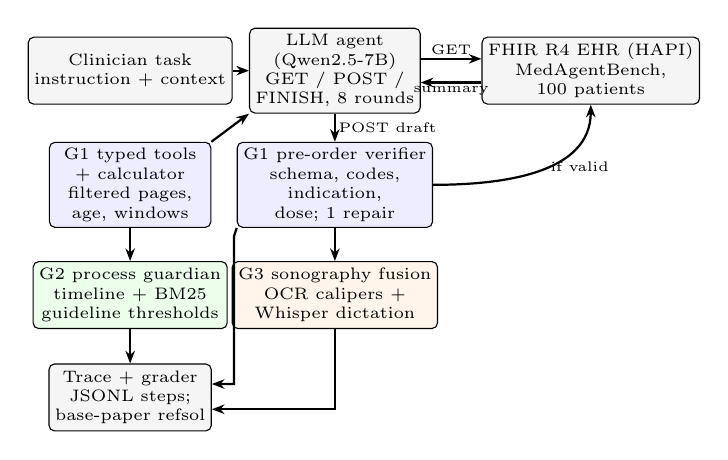
\begin{tikzpicture}[
  font=\fontsize{6}{7}\selectfont,
  box/.style={draw, rounded corners=2pt, align=center, minimum width=2.05cm, minimum height=0.85cm, inner sep=2.2pt, fill=gray!8},
  g1/.style={box, fill=blue!7}, g2/.style={box, fill=green!8}, g3/.style={box, fill=orange!8},
  arr/.style={-{Stealth[length=1.6mm]}, thick},
  lab/.style={font=\fontsize{5}{6}\selectfont, inner sep=1pt}]
\node[box] (task) at (0,0) {Clinician task\\instruction + context};
\node[box] (agent) at (2.6,0) {LLM agent\\(Qwen2.5-7B)\\GET / POST /\\FINISH, 8 rounds};
\node[box] (ehr) at (5.85,0) {FHIR R4 EHR (HAPI)\\MedAgentBench,\\100 patients};
\node[g1] (tools) at (0,-1.45) {G1 typed tools\\+ calculator\\filtered pages,\\age, windows};
\node[g1] (ver) at (2.6,-1.45) {G1 pre-order verifier\\schema, codes,\\indication,\\dose; 1 repair};
\node[g2] (pg) at (0,-2.85) {G2 process guardian\\timeline + BM25\\guideline thresholds};
\node[g3] (sono) at (2.6,-2.85) {G3 sonography fusion\\OCR calipers +\\Whisper dictation};
\node[box] (trace) at (0,-4.15) {Trace + grader\\JSONL steps;\\base-paper refsol};
\draw[arr] (task) -- (agent);
\draw[arr] ([yshift=1.5mm]agent.east) -- node[lab, above]{GET} ([yshift=1.5mm]ehr.west);
\draw[arr] ([yshift=-1.5mm]ehr.west) -- node[lab, below]{summary} ([yshift=-1.5mm]agent.east);
\draw[arr] (tools.north east) -- (agent.south west);
\draw[arr] (agent) -- node[lab, right]{POST draft} (ver);
\draw[arr] (ver.east) to[out=0, in=-90] node[lab, right, pos=0.55]{if valid} (ehr.south);
\draw[arr] (tools) -- (pg);
\draw[arr] (ver) -- (sono);
\draw[arr] (pg) -- (trace);
\draw[arr] (sono.south) |- ([yshift=-1.5mm]trace.east);
\draw[arr] (ver.south west) -- (1.32,-2.1) -- (1.32,-3.98) -- ([yshift=1.7mm]trace.east);
\end{tikzpicture}
\caption{MedGuardian wraps a single Qwen2.5-7B agent loop (top) with three switchable components. Gap 1's typed tools and calculator feed the agent and route its draft orders through a pre-order verifier that sits between the agent and the EHR, repairing or blocking a draft before it is executed; Gap 2's process guardian and Gap 3's sonography fusion consume the same task context off the main loop. Every step is written to a trace that the base paper's own grader scores only after the fact.}
\label{fig:arch}
\end{figure}

A single LLM agent (Qwen2.5-7B-Instruct \cite{qwen2025qwen25}) loops over GET, POST and FINISH against the EHR exactly as in the base paper. MedGuardian wraps this loop with three components, each switchable through a single configuration object so that any subset can be disabled independently for the ablation in Section~\ref{sec:ablation} (Fig.~\ref{fig:arch}). Every step---what was sent, what came back, timing and token counts---is written to a JSONL trace, so the comparisons in Section~\ref{sec:failure} can replay a run exactly.

\subsection{Gap 1: Deterministic Tools and Pre-Order Verification}
The typed FHIR tools follow every result page and return only the fields relevant to the task, sorted newest first, instead of handing the agent a raw bundle. Raw bundles inflate the conversation substantially: E2 averages 23,659 prompt tokens per task against 8,666 for E3. The tools also rewrite malformed date-range queries (\texttt{date=A/B} is rewritten to \texttt{date=geA\&date=leB}) and attach a concrete hint to any HTTP 400 response. A calculator layer derives facts the model otherwise computes unreliably: age as of the task's stated ``now,'' hours elapsed since an observation, and the count, mean or most recent value within a requested time window \cite{goodell2025calculations}; dosing-relevant renal function is obtained with Cockcroft--Gault \cite{cockcroft1976crcl} and CKD-EPI 2021 \cite{inker2021ckdepi}, and a drug-label lookup uses BM25 retrieval \cite{robertson2009bm25}.

The pre-order verifier runs every draft POST through six checks: \emph{structure} (right endpoint and resource type, with the required fields present, matched against the published FHIR function schemas); \emph{identity} (the patient in the request matches the task's MRN); \emph{coding} (the NDC, LOINC, SNOMED, or flowsheet code named in the task text, paired with the right code system); \emph{timing} (dates resolved exactly to ISO form---``next day at 8 am'' has to resolve to an actual timestamp, not just a loose phrase); \emph{indication} (the lab value that's supposed to trigger the order is checked live against the FHIR server---for instance, an order for magnesium gets blocked if there's no magnesium reading in the last 24 hours); and \emph{dose} (the dose is recomputed from whatever protocol the task itself states, e.g.\ tiered magnesium at 1/2/4 g, or potassium at 10 mEq per 0.1 below 3.5).

A draft that fails any check is never sent; the model receives the problem list and one repair attempt, in the spirit of self-refinement \cite{madaan2023selfrefine} but with deterministic, rule-based feedback rather than self-critique; a draft that is not clinically indicated at all is blocked outright. The same layer gives one retry when a reply is not a valid action, and recovers an action that the model wrapped in prose instead of emitting directly.

It must be stated explicitly that the verifier sits between the model and the EHR: the grader only ever scores what was actually sent, while every draft and every piece of feedback is preserved in the trace. Verifier rules are derived only from each task's own text, the published FHIR function schemas, and live FHIR data---never from the grader itself, which the verifier never has access to.

\subsection{Gap 2: Process Guardian}
The process guardian builds a timeline of doses, labs and procedure start/end times from the patient's FHIR resources, computing creatinine clearance with Cockcroft--Gault \cite{cockcroft1976crcl} where an interval (e.g.\ a direct oral anticoagulant's hold time) depends on renal function. Four checks are applied to this timeline, and their thresholds are read from a retrieved guideline chunk rather than hard-coded: BM25 retrieval \cite{robertson2009bm25} over an 18-chunk corpus summarising the PAUSE study \cite{douketis2019pause} and the 2022 ACCP perioperative guideline \cite{douketis2022accp} supplies, for example, a minimum hold of 24 or 48 hours for apixaban before low- or high-bleeding-risk procedures respectively, at least 120 hours for warfarin, an INR of at most 1.5 within 48 hours, and a platelet count of at least $50\times10^{9}$/L within 7 days.

Each flag carries a rule-based severity (interval violations are high around high-bleeding-risk procedures and medium otherwise; an out-of-range lab is high; a missing lab is medium), the supporting evidence, and the guideline citation it was checked against. Because thresholds come from retrieval rather than a fixed lookup table, the same checks resolve brand names (e.g.\ Eliquis for apixaban) and records where the bleeding-risk label itself is missing.

\subsection{Gap 3: Sonography Report Fusion}
The sonography pipeline reads on-screen caliper labels from the ultrasound screenshot with OCR (Apple Vision); the accompanying dictation is transcribed with Whisper base.en \cite{radford2023whisper}, and an LLM then fills a fixed report template from that transcript, constrained to valid JSON, with any invalid value dropped. Numeric fields are taken from the image, qualitative findings from the dictation, and a number reported by both sources that differs by more than 0.15 is flagged as a conflict for the radiologist to resolve, following structured-reporting practice \cite{esr2018structured}.

\subsection{Switchable Components}
Typed tools, the calculator, the order verifier, the process guardian's retrieval step, and each sonography modality are each a single configuration flag on \texttt{MedGuardianConfig}. The ablation in Section~\ref{sec:ablation} disables exactly one flag at a time to attribute MedGuardian's gain to each component individually.

\section{Experimental Setup}\label{sec:setup}

\begin{table}[t]
\centering
\small
\caption{Experimental setup: benchmark, splits, models, decoding parameters and hardware used for every run reported in this paper.}
\label{tab:setup}
\begin{tabular}{@{}l>{\raggedright\arraybackslash}p{5.1cm}@{}}
\toprule
\textbf{Item} & \textbf{Setting} \\
\midrule
Benchmark & MedAgentBench \texttt{test\_data\_v2} (300 tasks, 10 categories) \\
Splits & dev 20 (2/category), test 50 (5/category), seed 0 \\
Agent model & Qwen2.5-7B-Instruct Q4\_K\_M (Ollama 0.40.15) \\
Fidelity model & Mistral-7B-Instruct-v0.3 Q4\_K\_M \\
Decoding & temperature 0, max 2048 tokens, seed 0, context 16,384 \\
Protocol & GET / POST / FINISH, 8 rounds, base-paper grader \\
Gap 2 data & 30 test + 10 dev synthetic FHIR records \\
Gap 3 data & 20 test + 5 dev synthetic cases (image + audio) \\
Hardware & Apple M4, 16 GB unified memory, no GPU server, no API \\
\bottomrule
\end{tabular}
\end{table}

\textbf{Data and splits.} We use MedAgentBench's \texttt{test\_data\_v2} (300 tasks). Fixed, stratified splits with seed 0 give a 20-task development split (2 tasks per category) used for all tuning, and a 50-task test split (5 per category) touched once per configuration (Table~\ref{tab:setup}). A 50-task subset was chosen so every configuration could be run end-to-end on a single laptop; exact $n$ and confidence intervals are reported with every result.

\textbf{Gap datasets.} For Gap 2, MedGuardian-Timeline provides 30 test and 10 development FHIR-style records across six drugs at low or high bleeding risk; 12 of the 30 test records carry an injected violation (14 gold labels in total: 6 hold-too-short, 4 lab-out-of-range, 2 restart-too-early, 2 missing-lab), alongside a ``messy'' copy of the same 30 records using brand names and no explicit bleeding-risk label. Violations are injected by construction and gold labels are written by the generator, which never calls the guardian itself, correcting the circular evaluation of our Phase 1 proposal. For Gap 3, MedGuardian-Sono provides 20 test and 5 development cases, each a rendered ultrasound screenshot with 3--4 caliper measurements paired with a dictation spoken by one of four macOS voices with partial overlap between the two channels; 4 of the 20 test cases contain a deliberately mis-spoken number.

\textbf{Models and settings.} Qwen2.5-7B-Instruct Q4\_K\_M \cite{qwen2025qwen25} is used for every agent run; Mistral-7B-Instruct-v0.3 Q4\_K\_M \cite{jiang2023mistral} is used only for the fidelity check (E0). All runs use Ollama 0.40.15 with a 16,384-token context, temperature 0, a maximum of 2,048 output tokens, seed 0, and the base paper's 8-round cap, left unmodified. The hardware is a single Apple M4 laptop with 16 GB of unified memory, with the FHIR server running in Docker under Rosetta; no run ever calls an external API.

\textbf{Baselines and systems.} E1 is a non-agentic retrieve-then-answer pipeline: in one fixed step it retrieves the patient and every lab code named in the task, then the model produces all the orders and the FINISH answer together in a single call, with no loop, feedback, calculator, or verifier involved. An initial one-round design couldn't succeed by construction and was replaced after a dev-split check (Section~\ref{sec:failure}). E2 reproduces the base paper's agent with its unmodified prompt and protocol on our split. E3 is MedGuardian: the same model, prompt, round budget and grader as E2, plus the Gap 1 components of Section~\ref{sec:system}. Numbers for Llama-3.3-70B, Qwen2.5-72B and Claude 3.5 Sonnet v2 are reported from the base paper, not reproduced, since a 70B-class model does not fit in 16 GB.

\textbf{Harness.} We re-implemented the base paper's agent loop in-process rather than running it through AgentBench \cite{liu2024agentbench} itself, which pins an older Python version, carries a known bug, and offers no switches for component-level ablation. The base paper's own prompt (parsed from its released source), its HTTP helper and its grader are reused unchanged; E0, in Section~\ref{sec:eval}, is our fidelity evidence that this re-implementation behaves as the original harness would.

\section{Evaluation Methodology}\label{sec:eval}

\textbf{Benchmark metrics.} In general, query and action SR are all calculated with the base paper's own grader. We report 95\% Wilson confidence intervals throughout. E2 and E3 are compared on the same 50 tasks with the exact McNemar test \cite{mcnemar1947}, which is more powerful than comparing two independent proportions because it uses the paired, task-level outcomes directly.

\textbf{Gap metrics.} For Gap 2 we report micro precision, recall and F1 over (record, discrepancy type, item) triples, a false-alert rate (the share of clean records that receive any flag), and a severity-weighted miss rate (high severity weighted 3, medium 2, low 1). For Gap 3 we report field-level precision, recall and F1 (a numeric field counts as correct within 0.05, a categorical field only on an exact match), a measurement transcription error rate, conflict-detection precision and recall, BLEU-4 of the rendered report, and ASR word error rate.

\textbf{Fidelity of the comparison.} We are explicit about which numbers are ours and which are the base paper's: Llama-3.3-70B, Qwen2.5-72B and Claude 3.5 Sonnet v2 are reported figures taken directly from MedAgentBench, while every Qwen2.5-7B and Mistral-7B number in this paper is reproduced on our own split with our own harness. Our Mistral-7B v0.3 fidelity run (E0) gives 5.0 / 10.0 / 0.0\% overall/query/action on 20 tasks, against the base paper's 4.00 / 8.00 / 0.00\% on its full 300, which supports treating our harness as faithful to the original protocol. Because decoding at temperature 0 is deterministic in our setup---rerunning E3 produced byte-for-byte identical trajectories---we couldn't measure run-to-run variance this way, so we measured it separately at temperature 0.7 across 3 seeds instead (E6, Section~\ref{sec:ablation}). One more wrinkle: Ollama silently truncates any prompt that exceeds the context window we configured. Rather than let a truncated conversation get graded as if the agent had simply answered wrong, we detect this condition ourselves and score it the same way the base paper scores its own context-limit failures.

\begin{figure}[t]
\centering
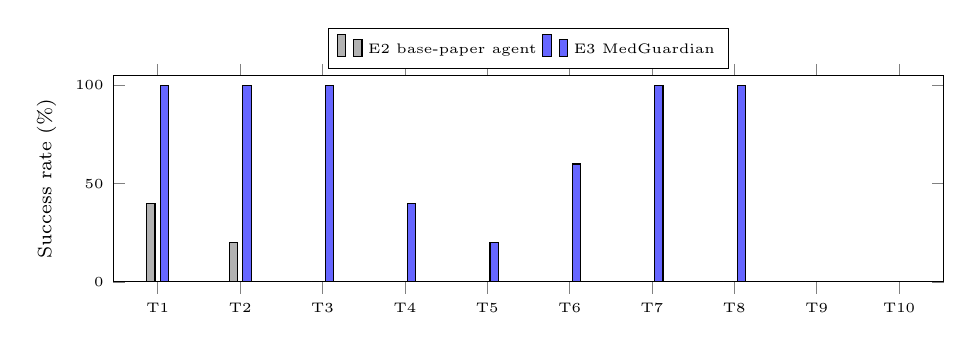
\begin{tikzpicture}
\begin{axis}[
  ybar, bar width=3pt, width=\columnwidth, height=4.2cm,
  symbolic x coords={T1,T2,T3,T4,T5,T6,T7,T8,T9,T10}, xtick=data,
  ymin=0, ymax=105, ytick={0,50,100}, ylabel={Success rate (\%)},
  tick label style={font=\tiny}, label style={font=\scriptsize},
  legend style={font=\tiny, at={(0.5,1.03)}, anchor=south, legend columns=2},
  enlarge x limits=0.06]
\addplot[fill=gray!60] coordinates {(T1,40) (T2,20) (T3,0) (T4,0) (T5,0) (T6,0) (T7,0) (T8,0) (T9,0) (T10,0)};
\addplot[fill=blue!60] coordinates {(T1,100) (T2,100) (T3,100) (T4,40) (T5,20) (T6,60) (T7,100) (T8,100) (T9,0) (T10,0)};
\legend{E2 base-paper agent, E3 MedGuardian}
\end{axis}
\end{tikzpicture}
\caption{Success rate per MedAgentBench task category on the 50-task test split (5 tasks per category), comparing the base-paper agent (E2) with MedGuardian (E3). The task8 value is not given directly in the running text; it is worked back from the reported action-SR total, the only value consistent with that total.}
\label{fig:per_category}
\end{figure}

\section{Results}\label{sec:results}

\begin{table*}[t]
\centering
\small
\caption{Success rate (\%) of models reported in the base paper and of the systems we reproduce or introduce, on the same 50-task test split; CIs are 95\% Wilson intervals; the bottom row reports the exact McNemar test comparing E2 and E3 on paired outcomes.}
\label{tab:main_results}
\begin{tabular}{lrcccccc}
\toprule
\textbf{System} & \textbf{Source} & $n$ & \textbf{Overall SR} & \textbf{95\% CI} & \textbf{Query SR} & \textbf{Action SR} \\
\midrule
Claude 3.5 Sonnet v2 & reported & 300 & 69.67 & -- & 85.33 & 54.00 \\
Qwen2.5-72B & reported & 300 & 51.33 & -- & 38.67 & 64.00 \\
Llama 3.3 70B & reported & 300 & 46.33 & -- & 50.00 & 42.67 \\
Mistral v0.3 7B & reported & 300 & 4.00 & -- & 8.00 & 0.00 \\
\midrule
E0 Mistral-7B v0.3 (base-paper agent) & reproduced & 20 & 5.0 & [0.9, 23.6] & 10.0 & 0.0 \\
E1 Qwen2.5-7B retrieve-then-answer (non-agentic) & reproduced & 50 & 32.0 & [20.8, 45.8] & 24.0 & 40.0 \\
E2 Qwen2.5-7B base-paper agent & reproduced & 50 & 6.0 & [2.1, 16.2] & 12.0 & 0.0 \\
E3 Qwen2.5-7B MedGuardian & reproduced & 50 & \textbf{62.0} & [48.2, 74.1] & \textbf{80.0} & \textbf{44.0} \\
\bottomrule
\multicolumn{7}{l}{E2 vs E3, exact McNemar: 0 tasks only E2 solved, 28 only E3 solved, $p=7.5\times10^{-9}$} \\
\end{tabular}
\end{table*}

\begin{table*}[t]
\centering
\small
\caption{Resolution of the three research gaps defined in Phase 1 against the hypothesis thresholds of Section~\ref{sec:problem}; the base-paper column lists the only directly comparable number MedAgentBench reports, or, where it reports none, our weakest evaluated baseline.}
\label{tab:gap_resolution}
\begin{tabular}{@{}>{\raggedright\arraybackslash}p{2.6cm}>{\raggedright\arraybackslash}p{3.4cm}>{\raggedright\arraybackslash}p{2.7cm}>{\raggedright\arraybackslash}p{3.0cm}>{\raggedright\arraybackslash}p{1.3cm}>{\raggedright\arraybackslash}p{3.0cm}@{}}
\toprule
\textbf{Gap} & \textbf{Method / component} & \textbf{Metric} & \textbf{Base paper result} & \textbf{Ours} & \textbf{Addressed?} \\
\midrule
Gap 1: action reliability & Typed FHIR tools, calculator, pre-order verifier & Action SR (\%), test 50 & 0.0 (E2, reproduced) & 44.0 (E3) & Fully ($\Delta$44.0 pp; H1: $\geq$+15) \\
Gap 2: process guardian & Timeline verifier + BM25 guideline retrieval & F1, 30 synthetic records & not evaluated (LLM-only arm: 0.31) & 1.00 & Fully (H2: F1$\geq$0.80, $\Delta\geq$+0.15) \\
Gap 3: sonography fusion & OCR + ASR + template-constrained fusion & Field F1, 20 synthetic cases & not evaluated (best unimodal: 0.83) & 1.00 & Fully (H3: fused $>$ both) \\
\bottomrule
\end{tabular}
\end{table*}

\subsection{Comparison with the Base Paper (E0--E3)}
Table~\ref{tab:main_results} lays out every system on the same 50-task test split, alongside the figures MedAgentBench itself reports across its full set of 300. The non-agentic baseline E1 reaches 32.0\% overall (query 24.0, action 40.0), showing what a single well-retrieved call can do without an agentic loop, feedback or verification. E2, the unmodified base-paper agent run with Qwen2.5-7B, reaches 6.0\%/12.0\%/0.0\% overall/query/action (95\% CI [2.1, 16.2]), close to the base paper's own 7B-class result for Mistral (4.00\%) and far below its large reported models. E3, MedGuardian, reaches 62.0\%/80.0\%/44.0\% (95\% CI [48.2, 74.1]); the exact McNemar test on E2 versus E3 finds 0 tasks solved only by E2 against 28 solved only by E3 ($p=7.5\times10^{-9}$). For context only, since the backbone and parameter count differ and we make no claim of beating these models: E3 with a 7B backbone finishes above the reported Llama-3.3-70B (46.33\%) and Qwen2.5-72B (51.33\%), and below Claude 3.5 Sonnet v2 (69.67\%).

On inspection, 7 of these 10 remaining failures had the correct underlying value but the wrong answer shape (a full sentence, or a list such as \texttt{[4.0, "2023-...", ...]} where a bare \texttt{[4.0]} was expected; for task10 specifically, a JSON object where a two-element list was expected). In 3 further task10 cases no recent HbA1c existed and the correct behaviour was to order one, but the agent answered \texttt{[-1]} without issuing the order, and in one task9 case the POST itself was written inside the FINISH answer instead of being sent. These remaining failures, then, are more a matter of answer formatting and order-decision behaviour than of data retrieval.

\subsection{Gap 1: Action Reliability (E4-G1)}
Action SR climbs from 0.0\% under E2 to 44.0\% under E3---a jump of +44.0 percentage points against the +15-point target we'd pre-registered for H1. The E3 trace backs this up directly: 10 draft orders were caught and rejected by the verifier across 10 tasks, every single one of them repaired successfully on the second attempt, and none were blocked outright as clinically unnecessary. \textbf{H1 is met.}

\subsection{Gap 2: Process Guardian (E4-G2)}
Table~\ref{tab:ablation} compares the full process guardian against an LLM-plus-retrieval arm and an LLM-only arm, on both the clean record set and a ``messy'' version of it. The guardian hits a precision of 1.00, a recall of 1.00, and an F1 of 1.00, with a false-alert rate and a severity-weighted miss rate both at 0.00; the LLM-plus-RAG arm manages F1 0.33 and the LLM-only arm F1 0.31. The ordering holds on the messy records too (guardian F1 1.00; LLM-plus-RAG 0.34; LLM-only 0.26). Retrieval roughly doubles the LLM-only arm's recall but close to triples its false-alert rate. \textbf{H2 is met}: F1~$\geq$~0.80, and the guardian improves on the LLM-only arm by well over the required 0.15 F1. It must be said plainly that the generator and the guideline corpus share one clinical source, so the guardian's score on clean records is best read as an upper bound; the LLM-only and LLM-plus-RAG arms, and the messy-record results, are the more informative comparison.

\subsection{Gap 3: Sonography Fusion (E4-G3)}
Field-level F1 is 0.60 for image-only, 0.83 for dictation-only, and 1.00 for the fused pipeline; measurement transcription error is 0.0, 0.10 and 0.0 respectively; conflict-detection precision and recall are 1.00 and 1.00; BLEU-4 is 16.5, 74.4 and 99.3; ASR word error rate over the 20 test cases is 6.2\%. \textbf{H3 is met}: fusion outperforms both single-source arms on field-level F1.

\subsection{Gap-Resolution Summary}
Table~\ref{tab:gap_resolution} summarises all three gaps against the base paper's only directly comparable figure (or, where none exists, our weakest baseline) and marks each ``Addressed?'' column using the hypothesis thresholds of Section~\ref{sec:problem}. All three gaps are resolved \textbf{Fully} by this criterion; none is only partially addressed.

\section{Ablation and Efficiency Analysis}\label{sec:ablation}

\begin{table}[t]
\centering
\small
\caption{Effect of removing one MedGuardian component at a time. Gap 1 rows use the 20-task development split (5 points per task); Gap 2 and Gap 3 rows use their own 30- and 20-case test sets, with Gap 2 also reported on a lexically perturbed (``messy'') copy of the same records.}
\label{tab:ablation}
\setlength{\tabcolsep}{4pt}
\begin{tabular}{lcccc}
\toprule
\textbf{Configuration} & \textbf{Overall} & \textbf{Query} & \textbf{Action} & $\boldsymbol{\Delta}$ \\
\midrule
G1: MedGuardian (all) & 80.0 & 100.0 & 60.0 & -- \\
G1: $-$ typed FHIR tools & 25.0 & 10.0 & 40.0 & $-55.0$ \\
G1: $-$ calculator & 55.0 & 50.0 & 60.0 & $-25.0$ \\
G1: $-$ order verifier & 60.0 & 100.0 & 20.0 & $-20.0$ \\
G1: base-paper agent (all off) & 5.0 & 10.0 & 0.0 & $-75.0$ \\
\bottomrule
\end{tabular}

\vspace{4pt}
\begin{tabular}{lccc}
\toprule
\textbf{Configuration} & \textbf{F1} & \textbf{P} & \textbf{R} \\
\midrule
G2: timeline verifier + RAG & 1.00 & 1.00 & 1.00 \\
G2: $-$ timeline verifier (LLM+RAG) & 0.33 & 0.23 & 0.57 \\
G2: $-$ verifier $-$ RAG (LLM only) & 0.31 & 0.33 & 0.29 \\
G2: messy, guardian & 1.00 & 1.00 & 1.00 \\
G2: messy, LLM+RAG & 0.34 & 0.24 & 0.57 \\
G2: messy, LLM only & 0.26 & 0.24 & 0.29 \\
\bottomrule
\end{tabular}

\vspace{4pt}
\begin{tabular}{lcc}
\toprule
\textbf{Configuration} & \textbf{Field F1} & \textbf{BLEU-4} \\
\midrule
G3: fused & 1.00 & 99.3 \\
G3: $-$ image OCR (dictation only) & 0.83 & 74.4 \\
G3: $-$ dictation ASR (image only) & 0.60 & 16.5 \\
\bottomrule
\end{tabular}
\end{table}

\begin{table}[t]
\centering
\small
\caption{Cost and reliability per task on the 50-task test split (Apple M4, 16 GB, Qwen2.5-7B-Instruct Q4\_K\_M, zero API spend); the bottom row is mean $\pm$ SD overall success rate for MedGuardian at temperature 0.7 over three seeds on a 10-task development subset.}
\label{tab:efficiency}
\setlength{\tabcolsep}{3.5pt}
\begin{tabular}{lccccccc}
\toprule
\textbf{Sys.} & \textbf{p50} & \textbf{p95} & \textbf{tok.in} & \textbf{tok.out} & \textbf{rnds} & \textbf{GET/cor.} & \textbf{fail.} \\
\midrule
E2 & 57 & 344 & 23,659 & 525 & 5.40 & 79.3 & 28/50 \\
E3 & 93 & 200 & 8,666 & 160 & 2.22 & 1.3 & 0/50 \\
\bottomrule
\multicolumn{8}{l}{E6, T=0.7, 3 seeds, dev-10: overall SR 73.3 $\pm$ 15.3} \\
\end{tabular}
\end{table}

\textbf{Gap 1 ablation (E5, development split).} Table~\ref{tab:ablation} removes one Gap 1 component at a time from the full configuration (80.0\% overall on dev-20). Removing the typed FHIR tools drops overall SR to 25.0\% (7 of 20 tasks then hit the round limit, and prompt tokens roughly double); removing the calculator drops it to 55.0\% (query SR falls from 100 to 50\% while action SR is unaffected); removing the order verifier drops it to 60.0\% (query SR is unaffected while action SR falls from 60 to 20\%); disabling all three components at once reproduces the base-paper agent at 5.0\%. Each component's loss, in other words, lands on the task type it was built for: the typed tools and the calculator chiefly protect query tasks, and the verifier chiefly protects action tasks. Because this split has only 20 tasks, each one is worth 5 percentage points, and these figures should be read with that granularity in mind.

\textbf{Gap 2 and Gap 3 ablation.} For these two gaps the E4 arms already reported in Section~\ref{sec:setup} are the ablation: removing the timeline verifier leaves an LLM-plus-RAG arm, and removing retrieval as well leaves an LLM-only arm; removing OCR leaves a dictation-only arm and removing ASR leaves an image-only arm (Table~\ref{tab:ablation}).

\textbf{Efficiency (E6).} Table~\ref{tab:efficiency} reports median and 95th-percentile latency, prompt and output tokens, rounds used, and GET calls per correct task for E2 and E3. E3 is slower than E2 at the median (93 vs 57 s/task, reflecting the verifier's extra calls and repair rounds) but much cheaper in tokens (8,666 vs 23,659 prompt tokens per task, 160 vs 525 output tokens) and in GET calls per correct task (1.3 vs 79.3), and no E3 run exhausts the round budget against 28 of 50 for E2. Since neither system ever calls a paid API, none of this costs anything in dollar terms---we report wall-clock time on the M4 instead, and measured a throughput of about 127 tokens/s on the prompt and 15 tokens/s during generation.

\textbf{Reliability.} The bottom row of Table~\ref{tab:efficiency} reports MedGuardian's overall SR at temperature 0.7 over 3 seeds on a 10-task development subset: 73.3 $\pm$ 15.3. Individually, the three seeds gave 70, 90 and 60\%; task10-22 failed under every seed, and task2-18 and task9-18 failed under two of the three. A single 10-task sample can therefore move by 30 points between seeds, which is why we treat our temperature-0 test-split result as a point estimate and report its Wilson confidence interval rather than a single number without uncertainty.

\section{Failure Analysis}\label{sec:failure}

\begin{table}[t]
\centering
\small
\caption{Automatically bucketed failure categories on the 50-task test split for MedGuardian (E3) and the unmodified base-paper agent (E2); categories are assigned by first match in a fixed rule list, with a sample of each hand-checked.}
\label{tab:failures}
\begin{tabular}{llrr}
\toprule
\textbf{Run} & \textbf{Failure category} & $n$ & \textbf{Share} \\
\midrule
E3 & answer format & 9 & 47\% \\
E3 & time window error & 5 & 26\% \\
E3 & order decision & 5 & 26\% \\
E2 & round limit & 28 & 60\% \\
E2 & order payload or value & 10 & 21\% \\
E2 & wrong value & 7 & 15\% \\
E2 & order decision & 2 & 4\% \\
\bottomrule
\end{tabular}
\end{table}

\textbf{Categories and frequencies.} Table~\ref{tab:failures} buckets every test-split failure by first match in a fixed rule list (context overflow; round limit; invalid action; FHIR query error; an unnecessary POST on a query task; an order blocked; answer format, meaning the right value in the wrong shape; time window error, meaning a value reported from outside the requested window, or a reported $-1$ when a value existed; order decision, meaning no order or the wrong decision on an action task; and, last, order payload or value and plain wrong value, both checked against the grader's reference solution only after the run, never by the system itself). E3 has 19 failures in total: answer format 9, time window error 5, order decision 5. E2 has 47: round limit 28, order payload or value 10, wrong value 7, order decision 2. MedGuardian removes E2's dominant failure mode outright (round limit, 28 of 50 down to 0 of 50); what remains is concentrated in answer formatting and reading the calculator's time window, not in retrieving the underlying data.

\textbf{Representative trajectories.} \emph{Success, verifier repair} (task3-28, recording a blood pressure for a patient): the agent's first POST targeted the generic \texttt{.../fhir/} endpoint without a resource type; the verifier rejected it with an explicit reason and did not send it; the agent's second POST, to \texttt{.../fhir/Observation}, was accepted, and the task finished correctly. Ten such repairs occur on the test split, and all ten are graded correct; the same class of mistake reaches the EHR unchecked under the base-paper agent.

\emph{Success, typed tools on a query task} (task1-26, finding a patient's MRN by name and date of birth): both E2 and E3 issued the same raw name-based GET, which HAPI's partial name matching returns zero results for; E2 reported the patient as not found, while E3's typed tool split the name into given and family components, found the match, and answered correctly in two rounds.

\emph{Failure, answer format} (task5-28, asking for the most recent magnesium level and an order only if it is low): retrieval and the no-order decision were both correct, but the agent answered with a full sentence where the grader expects the bare value \texttt{[2.0]}; nine of nineteen E3 failures share this pattern, and we treat a stricter check on the FINISH format as future work rather than tuning further against this grader.

\emph{Failure, time window} (task4-1, asking for the most recent magnesium within the last 24 hours): the calculator correctly reported no reading inside the window, but the agent ignored it and answered with a 23-hour-old-plus reading instead of the expected \texttt{[-1]}; five of nineteen failures share this pattern, and a direct fix would let the calculator answer such window questions itself, or have the verifier check a FINISH value against the calculator's own window output.

\textbf{Iterative improvement.} Our development log tracks several fixes made along the way, each with a measurable payoff: we corrected the circular Gap 2 evaluation from Phase 1 by separating the violation generator from the guardian; fixing a power and swap-memory misconfiguration roughly tripled our throughput; we caught Ollama's silent prompt truncation and now count it explicitly as a context-limit outcome rather than scoring it as an ordinary failure; the base-paper agent's own dominant failure modes on the dev split were what pointed us toward building the three Gap 1 components in the first place; and a URL-encoding bug in date-range queries was found and fixed on the development split, before the test split was ever touched.

\section{Limitations and Threats to Validity}

Our test split has only 50 tasks, which is reflected in the width of the confidence intervals in Table~\ref{tab:main_results}; the Gap 2 and Gap 3 evaluation sets are smaller still, at 30 and 20 cases. We evaluate a single backbone, quantised to 4 bits, and do not reproduce the base paper's 70B and hosted-API models ourselves, since a 70B model does not fit in 16 GB; those numbers are reported figures, not ours. Our harness re-implements the base paper's loop in-process rather than running through AgentBench itself (Section~\ref{sec:system}); the E0 fidelity check (our Mistral-7B v0.3 at 5.0/10.0/0.0\%, $n=20$, against the base paper's 4.00/8.00/0.00\%, $n=300$) is our mitigation, not a guarantee of exact equivalence.

The Gap 1 verifier's rules were written from the benchmark's own task templates---the indication and dosing protocols stated in each task's text---so their generalisation to order types the benchmark does not cover is untested. For Gap 2, the record generator and the retrieval corpus were built from the same underlying clinical source, so the guardian's score on clean, well-formed records is best read as an upper bound rather than a general-population estimate; the LLM-only and LLM-plus-RAG arms and the messy-record results are the more informative comparison. The corpus's procedure keyword list was also written after seeing the generator's procedure names, which is a further source of optimism in the clean-record result, and it is a curated summary rather than a clinically validated guideline text.

For Gap 3, the ultrasound screenshots and dictation audio are both synthetic (the audio is text-to-speech with no accents, background noise or disfluency), and because the reports are rendered from a fixed template, BLEU-4 is best read as reflecting field-level correctness rather than free-text quality. No part of this evaluation includes a clinician review or Likert rating; this was part of our Phase 1 plan and was dropped for this phase because arranging clinician time was not feasible within a laptop-scale, single-term project, and we flag it as the most important piece of future validation. All measurements were taken on one fanless laptop, so latency in particular should be read as indicative rather than as a tight bound, since it can vary with the machine's thermal state. Finally, our Phase 1 proposal's reported 10-out-of-10 result used a Gap 2 evaluation in which the generator and the guardian shared logic; that result was circular and is superseded by the figures reported here.

\section{Conclusion}

Across all three Phase 1 gaps, deterministic, verifiable machinery around a small open-weight model closed most of the gap to the base paper's large models for the tasks that machinery targets. The action SR score rose by +44.0 points, far exceeding the +15.0-point target, by fixing or canceling draft orders before they're recorded, without altering the underlying model at all. A retrieval-grounded process guardian achieved an F1 of 1.00 compared to 0.31 for an LLM using only its own recalled thresholds rather than those specified in the guidelines. Fusing an on-screen measurement with a dictation, rather than trusting either alone, raised sonography field-F1 from 0.83 for the better single modality to 1.00.

These results suggest a larger conclusion: even though the model itself stays the same, a 7B model running on one laptop can be made significantly more reliable at acting on a clinical record just by adding deterministic tools and verification around it, without any extra API cost. Concrete next steps include testing on the benchmark's full 300 tasks and across more backbones; a clinician review of the Gap 2 guideline corpus and the Gap 3 report template; real, non-synthetic dictation audio; deriving the Gap 1 verifier's rules from FHIR schemas in a more general way so they apply to order types we haven't seen; and multi-seed reliability runs at the full test scale rather than on a 10-task subset.

\bibliographystyle{IEEEtran}
\bibliography{references}

\end{document}
